% Exact LaTeX recreation of the supplied Phase-1.pdf
% Compile with pdfLaTeX. Place member pictures in the same folder if required.

\documentclass[11pt,a4paper]{article}

\usepackage[a4paper,left=2.0cm,right=2.0cm,top=1.55cm,bottom=1.55cm]{geometry}
\usepackage[T1]{fontenc}
\usepackage{lmodern}
\usepackage{graphicx}
\usepackage{float}
\usepackage{xcolor}
\usepackage{array}
\usepackage{tabularx}
\usepackage{ragged2e}
\usepackage{enumitem}
\usepackage{fancyhdr}
\usepackage{tikz}
\usepackage{setspace}
\usepackage{url}

% -------------------------------------------------
% COLOURS
% -------------------------------------------------
\definecolor{TitleBlue}{RGB}{61,103,154}

% -------------------------------------------------
% GENERAL SETTINGS
% -------------------------------------------------
\setlength{\parindent}{0pt}
\setlength{\parskip}{0pt}
\renewcommand{\arraystretch}{1.0}

% The supplied document uses a clean sans-serif heading style
% and italic serif-style explanatory text.
\newcommand{\blueheading}[1]{%
    {\sffamily\color{TitleBlue}\fontsize{15}{18}\selectfont #1}%
}

\newcommand{\bluebigheading}[1]{%
    {\sffamily\bfseries\color{TitleBlue}\fontsize{16}{19}\selectfont #1}%
}

\newcommand{\instruction}[1]{%
    {\itshape\fontsize{10.5}{12.5}\selectfont #1}%
}

\newcommand{\answerbox}[2][3.0cm]{%
    \vspace{2pt}
    \noindent
    \fbox{%
        \begin{minipage}[t][#1][t]{\dimexpr\textwidth-2\fboxsep-2\fboxrule\relax}
            \vspace{1mm}
            \itshape #2
        \end{minipage}
    }
}

% -------------------------------------------------
% HEADER / FOOTER
% -------------------------------------------------
\pagestyle{fancy}
\fancyhf{}
\renewcommand{\headrulewidth}{0pt}
\renewcommand{\footrulewidth}{0pt}

\fancyhead[L]{%
    \sffamily\bfseries\itshape\fontsize{10.5}{12}\selectfont
    Data Structures and Programming in C++/DSCPP
}
\fancyhead[R]{%
    \sffamily\bfseries\fontsize{10.5}{12}\selectfont
    PROJECT PROPOSAL
}
\fancyfoot[R]{%
    \itshape\fontsize{10}{12}\selectfont
    Page \thepage
}
\setlength{\headheight}{14pt}
\setlength{\headsep}{23pt}
\setlength{\footskip}{24pt}

% -------------------------------------------------
% PAGE 1
% -------------------------------------------------
\begin{document}

\vspace*{4mm}

\bluebigheading{PROJECT AND TEAM INFORMATION}

\vspace{13mm}

\blueheading{Project Title}

\vspace{1mm}


\answerbox[1.0cm]{\bfseries\fontsize{12}{14}\selectfont
The Detective's Dossier: An Interactive 2D Murder Mystery and Investigation Game}

\vspace{13mm}

\blueheading{Student / Team Information}

\vspace{2mm}

% Team information table
% Compact 4-member layout so all members remain on Page 1.
\noindent
\begin{tabularx}{\textwidth}{|>{\RaggedRight\arraybackslash}p{0.58\textwidth}|>{\RaggedRight\arraybackslash}X|}
\hline
\begin{minipage}[t]{\linewidth}
\vspace{1.5mm}
\textit{Team Name:}\\[-1mm]
\textit{Team ID:}
\vspace{1.5mm}
\end{minipage}
&
\begin{minipage}[t]{\linewidth}
\vspace{1.5mm}
\textit{Code Detektives}\\[-1mm]
\textit{DSCPP-III-2026-T027}
\vspace{1.5mm}
\end{minipage}
\\
\hline
\begin{minipage}[t][3.8cm][t]{\linewidth}
\vspace{1.5mm}
\textbf{Team member 1 (Team Lead)}\\[-1mm]
\textit{(Last Name, name: student ID: email, picture):}
\vspace{2.0cm}
\end{minipage}
&
\begin{minipage}[t][3.8cm][t]{\linewidth}
\vspace{1.5mm}
\textit{Bahuguna, Ashutosh -- 2510370440}\\
\url{ashutoshbahuguna2468@gmail.com}

\vspace{2mm}
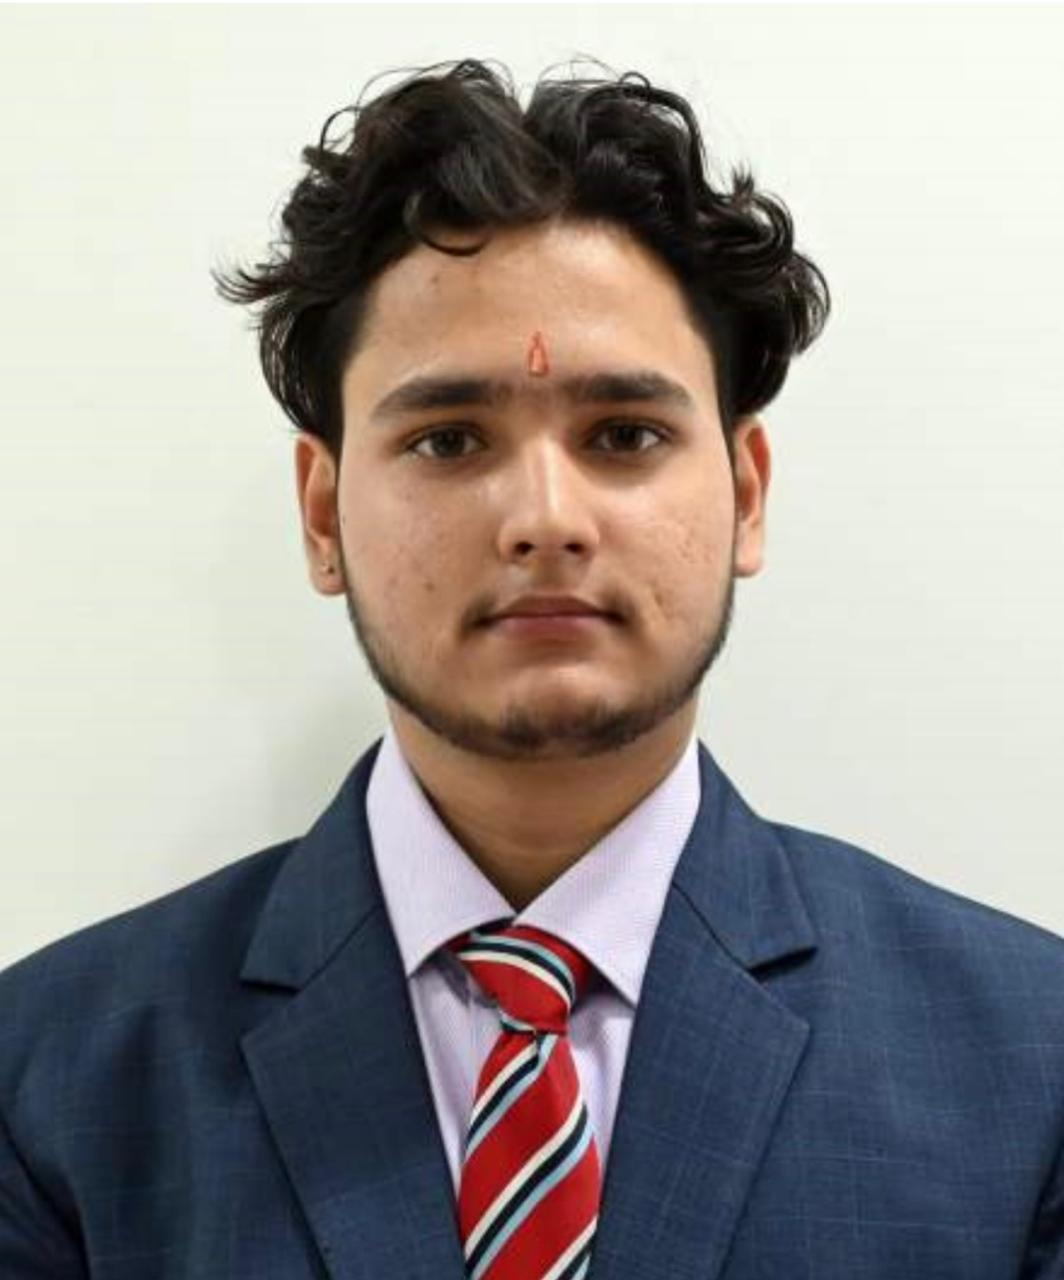
\includegraphics[width=3.0cm,height=1.5cm,keepaspectratio]{member1.jpeg}
\end{minipage}
\\
\hline
\begin{minipage}[t][3.8cm][t]{\linewidth}
\vspace{1.5mm}
\textbf{Team member 2}\\[-1mm]
\textit{(Last Name, name: student ID: email, picture):}
\vspace{2.0cm}
\end{minipage}
&
\begin{minipage}[t][3.8cm][t]{\linewidth}
\vspace{1.5mm}
\textit{Pundir, Snehal -- 2510370590}\\
\url{snehalpundir21052@gmail.com}

\vspace{2mm}
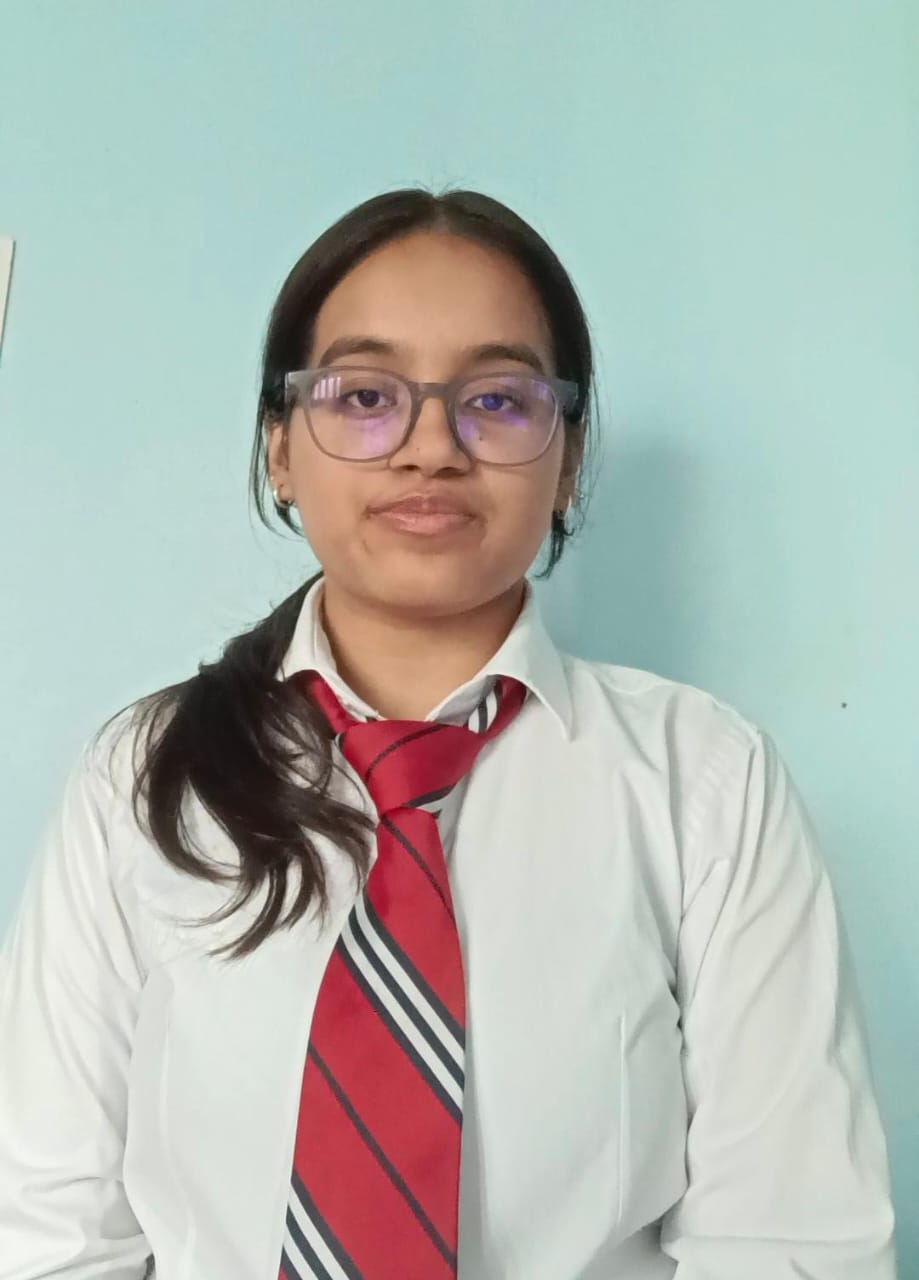
\includegraphics[width=3.0cm,height=1.5cm,keepaspectratio]{member2.jpeg}
\end{minipage}
\\
\hline
\begin{minipage}[t][3.8cm][t]{\linewidth}
\vspace{1.5mm}
\textbf{Team member 3}\\[-1mm]
\textit{(Last Name, name: student ID: email, picture):}
\vspace{2.0cm}
\end{minipage}
&
\begin{minipage}[t][3.8cm][t]{\linewidth}
\vspace{1.5mm}
\textit{Somraan, Vidhi -- 2510380302}\\
\url{Vidhisomraan@gmail.com}

\vspace{2mm}
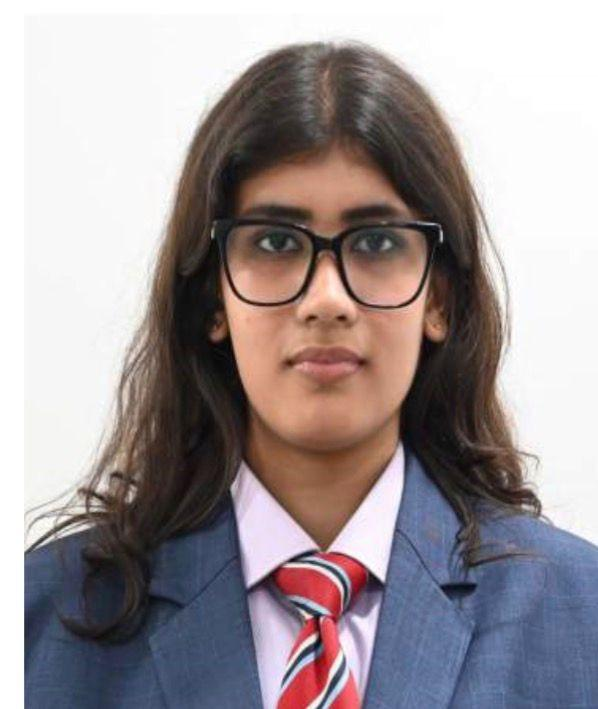
\includegraphics[width=3.0cm,height=1.5cm,keepaspectratio]{member3.jpeg}
\end{minipage}
\\
\hline

\end{tabularx}

\newpage

% -------------------------------------------------
% PAGE 2
% -------------------------------------------------

\bluebigheading{PROPOSAL DESCRIPTION (10 pts)}

\vspace{12mm}

\blueheading{Motivation (1 pt)}

\vspace{1mm}

\answerbox[6.1cm]{Mysteries and detective stories are always interesting because of the clues, the suspects, the observations and the logical reasoning. That is why we decided to create a project in the form of an interactive game.

In The Detective’s Dossier project players will take on the role of detectives in a 2D murder mystery game. They will explore the crime scenes, go to places of interest, find clues, examine the evidence and question the suspects. They will have to connect the clues in order to work out what had happened.

The primary reason for selecting the project was the chance to put Data Structures and Algorithms to practical use rather than using them individually in programming tasks. Several DSA concepts can be used in the investigation.Graphs can be employed to represent places of interest and the relationships between them, while BFS and DFS can be used for exploration and Dijkstra’s Algorithm can be used to calculate the paths between places.

That is to say, the game will have elements of a detective story and also include DSA concepts as well as C++ and OOP.}

\vspace{12mm}

\blueheading{State of the Art / Current solution (1 pt)}

\vspace{1mm}


\answerbox[7cm]{Already there are a large number of detective and murder mystery games in which the players have to investigate the cases, gather the clues and find out who the culprit is. The majority of these games feature a fixed storyline together with pre-determined characters, locations, dialogues and clues.

These games are primarily concerned with the story and providing entertainment, the actual relationships between the various clues, suspects, and locations usually being managed internally by the game.

In the project we aim to make the process of investigation more structured; the player will need to explore the case and use the information gathered during the investigation in order to reach a conclusion.

DSA will also play a direct role in the operation of the game: graphs can be used to represent locations and relationships, BFS and DFS can be applied to traversal, and Dijkstra’s algorithm can assist with navigation. Furthermore, hashing, stacks, queues, searching and sorting can all be used whenever they are useful.

It will enable us to bring together the fundamental concept of a detective game with the practical application of DSA.}

\vspace{12mm}
\newpage
\blueheading{Project Goals and Milestones (2 pts)}

\vspace{1mm}

\answerbox[21cm]{The aim of The Detective’s Dossier is to create a playable 2D murder mystery game using C++, object-oriented programming, data structures and algorithms, Qt and SQLite.

\textbf{Main Goals:}

\begin{itemize}[leftmargin=*, itemsep=2pt, topsep=2pt]
    \item Set up a 2D environment in which players can look into various murder cases.
    
    \item Let players explore different locations and gather clues and evidence.
    
    \item Permit interactions with the suspects via interrogation and conversations.
    
    \item Link the suspects, clues, evidence and locations in a way that makes sense.
    
    \item Include data structures and algorithms as an important element of the game logic.
    
    \item Organise the various game entities and modules using object-oriented programming concepts.
    
    \item Use SQLite to store cases, users, evidence, and progress.
    
    \item Let the player make their final accusation once the investigation has been completed.
    
    \item Provide a result that is suitable in accordance with the player's investigation and final choice.
\end{itemize}
\textbf{Milestones}

\vspace{3mm}

\textbf{Phase I -- Planning and Design}

\begin{itemize}[leftmargin=*, itemsep=2pt, topsep=2pt]
    \item Understand the problem and the requirements.
    \item Finish off the game concept and features.
    \item Choose the technologies and DSA concepts that are to be used.
    \item Draw up the system architecture and project design.
\end{itemize}

\vspace{2mm}

\textbf{Phase II -- Development}

\begin{itemize}[leftmargin=*, itemsep=2pt, topsep=2pt]
    \item Create the basic 2D interface based on Qt.
    \item Develop the C++ and object-oriented programming structure of the game.
    \item Build the needed DSA parts.
    \item Set up the SQLite database.
    \item Work on the key aspects of the investigation and gameplay.
\end{itemize}

\vspace{2mm}

\textbf{Phase III -- Integration and Testing}

\begin{itemize}[leftmargin=*, itemsep=2pt, topsep=2pt]
    \item Make sure that all the modules are connected.
    \item Add various murder cases and test them.
    \item Check the DSA implementations and the database.
    \item Investigate the entire game.
    \item Carry out user testing and make improvements to the final prototype.
\end{itemize}}

\vspace{12mm}
\newpage
\blueheading{Project Approach (3 pts)}

\vspace{1mm}


\answerbox[15.5cm]{\vspace{2mm}

\textbf{• User Interaction}

The player begins by using the login screen to enter the game and once logged in they will be able to start the investigation.

\vspace{2mm}

\textbf{• 2D Game Interface}

The graphical interface and the 2D game environment will be created using Qt. The program will have screens permitting selection of a case, exploration of the location, collection of evidence, interaction with suspects and the final resolution of the case.\vspace{2mm}

\textbf{• C++ and OOP}

The primary application will be developed using C++ and Object-Oriented Programming.

Various game elments such as users, cases, suspects, evidence and locations can be dealt by means of classes and objects and the code will be organized using encapsulation,inheritance and abstraction concepts.\vspace{2mm}

\textbf{• DSA-Driven Investigation}

Data Structures and Algorithms will form the basis of the investigation system.\vspace{2mm}

A graph can be used in order to show the connections between different locations and various relationships and BFS and DFS can be used to explore connected locations or investigation elements.\vspace{2mm}

Dijkstra's algorithm can be used for finding the shortest path between different locations and can be of assistance when analysing movement in a case.\vspace{2mm}

Hashing can be used in rapid search of suspects, evidences and other case details. Stacks can be used to keep track of the investigation history and to allow backtracking, while queues can be used for tasks which have to be dealt with in sequence.\vspace{2mm}

\textbf{• Database and Storage}

SQLite is to be used as the local database, and it will hold information on user accounts, cases, suspects, evidence, locations, relationships and player progress.

It will enable the game to save and retrieve the information when needed.\vspace{2mm}

\textbf{• Development and Testing}

The project will be carried out step by step by first creating and testing each module separately before integrating them.}


\newpage
% -------------------------------------------------
% PAGE 3
% -------------------------------------------------

\blueheading{System Architecture (High Level Diagram)(2 pts)}

\vspace{1mm}



\answerbox[3.5cm]{The system will be made up of four components: the Qt-based 2D Game Interface, the C++/OOP Application and Game Logic, the DSA & Algorithm Engine, and the SQLite Database.

The player will use the Qt interface to interact with the game, and the interface will communicate with the C++/OOP game logic, which in turn will control the various game activities.

The Algorithm Engine and DSA will carry out functions such as navigation, traversal, relationship analysis, and the management of searching and investigation history. Information concerning users, cases, suspects, evidence, locations and game progress will be stored in the SQLite database.}
 \vspace{2mm}
 \begin{figure}[H]
    \centering
    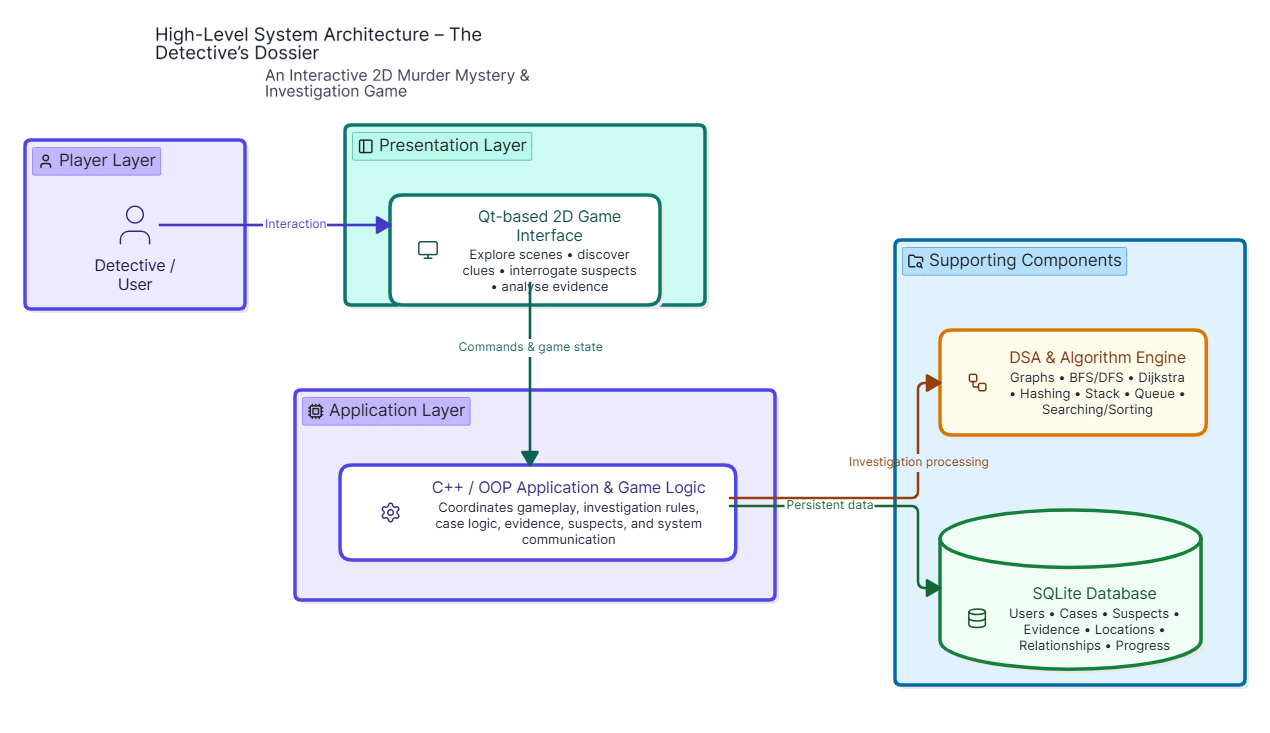
\includegraphics[
        width=\textwidth,
        height=25cm,
        keepaspectratio
    ]{architechture.png}
    \caption{High-Level System Architecture of The Detective's Dossier}
    \label{fig:architecture}
\end{figure}
\vspace{12mm}
\newpage
\blueheading{Project Outcome / Deliverables (1 pts)}

\vspace{1mm}

\answerbox[10cm]{The end result will be a fully functioning 2D murder mystery and detective investigation game, developed using C++, object-oriented programming, data structures and algorithms, Qt and SQLite.

The player can choose a case, investigate various locations, gather evidence, talk to the suspects, link the clues together and then make an accusation.

The project will also show the application of DSA concepts in a real-life situation rather than applying them independently just for academic purposes.

\vspace{2mm}

\textbf{Expected Deliverables}

\vspace{3mm}

\begin{itemize}[leftmargin=*, itemsep=2pt, topsep=2pt]

    \item A two-dimensional game interface based on Qt that is operational.

    \item A C++ application that makes use of object-oriented programming concepts.

    \item An investigation and navigation system based on DSA.

    \item An SQLite database for storing game information.

    \item A number of murder mystery cases that can be played.

    \item Interaction between suspects, evidence, clues and locations.

    \item The background of the investigation and the method used to solve the case.

    \item A system for the final accusation and the outcome of the case.

    \item A working prototype that has been tested and integrated.

\end{itemize}}

\vspace{12mm}

\blueheading{Assumptions}

\vspace{6mm}


\answerbox[6cm]{\begin{itemize}[leftmargin=1.5em, itemsep=4pt, topsep=0pt]

    \item The project will initially be developed as a 2D desktop application.

    \item The system will run on a computer that supports C++, Qt and SQLite.

    \item The development team will define the case details, suspects, clues and evidence used in the game.

    \item The required game information will be stored in a local SQLite database.

    \item An internet connection will not be required for the main gameplay.

    \item DSA concepts will be included based on their usefulness in the investigation rather than adding algorithms unnecessarily.

    \item The first version of the game will focus more on gameplay and investigation than on advanced 3D graphics.

\end{itemize}
}

\vspace{12mm}
\newpage
\blueheading{References}

\vspace{1mm}

\answerbox[5cm]{\begin{enumerate}[leftmargin=1.8em, itemsep=5pt, topsep=0pt]

    \item C++ Reference, cppreference:
    \texttt{https://en.cppreference.com/}

    \item Qt Documentation:
    \texttt{https://doc.qt.io/}

    \item SQLite Documentation:
    \texttt{https://www.sqlite.org/docs.html}

    \item T. H. Cormen, C. E. Leiserson, R. L. Rivest and C. Stein,
    \textit{Introduction to Algorithms}, MIT Press.

    \item R. Lafore,
    \textit{Object-Oriented Programming in C++}.

    \item Qt Creator Documentation:
    \texttt{https://doc.qt.io/qtcreator/}

\end{enumerate}}

\end{document}
